\documentclass[12pt,a4paper]{article}
\usepackage{times}
\usepackage{durhampaper}
\usepackage{url}
\usepackage{harvard}
\usepackage{cite}
\usepackage{graphicx}


\citationmode{abbr}
\bibliographystyle{plain}
\graphicspath{ {./images/} }

\title{Using Stereo Vision for Object Distance Ranging}
\author{} % leave; your name goes into \student{}
\student{Molly Hayward}

\date{20/11/2019}

\begin{document}

\maketitle

\vspace{3 mm}
\section{Introduction}
\noindent Producing accurate depth-estimation of objects is a complex problem in computer vision, as images often contain noise due to inconsistent illumination, object occlusion and challenging weather conditions. In this report, I detail my approach to integrating state-of-the-art object detection (YOLO) with dense stereo ranging, and a high-level overview of this solution is given in Figure 1.  I experimented with different implementations of stages 3-7 in order to improve performance under challenging conditions, and provide a comparative evaluation of these techniques in the remainder of the report.


\begin{center}
	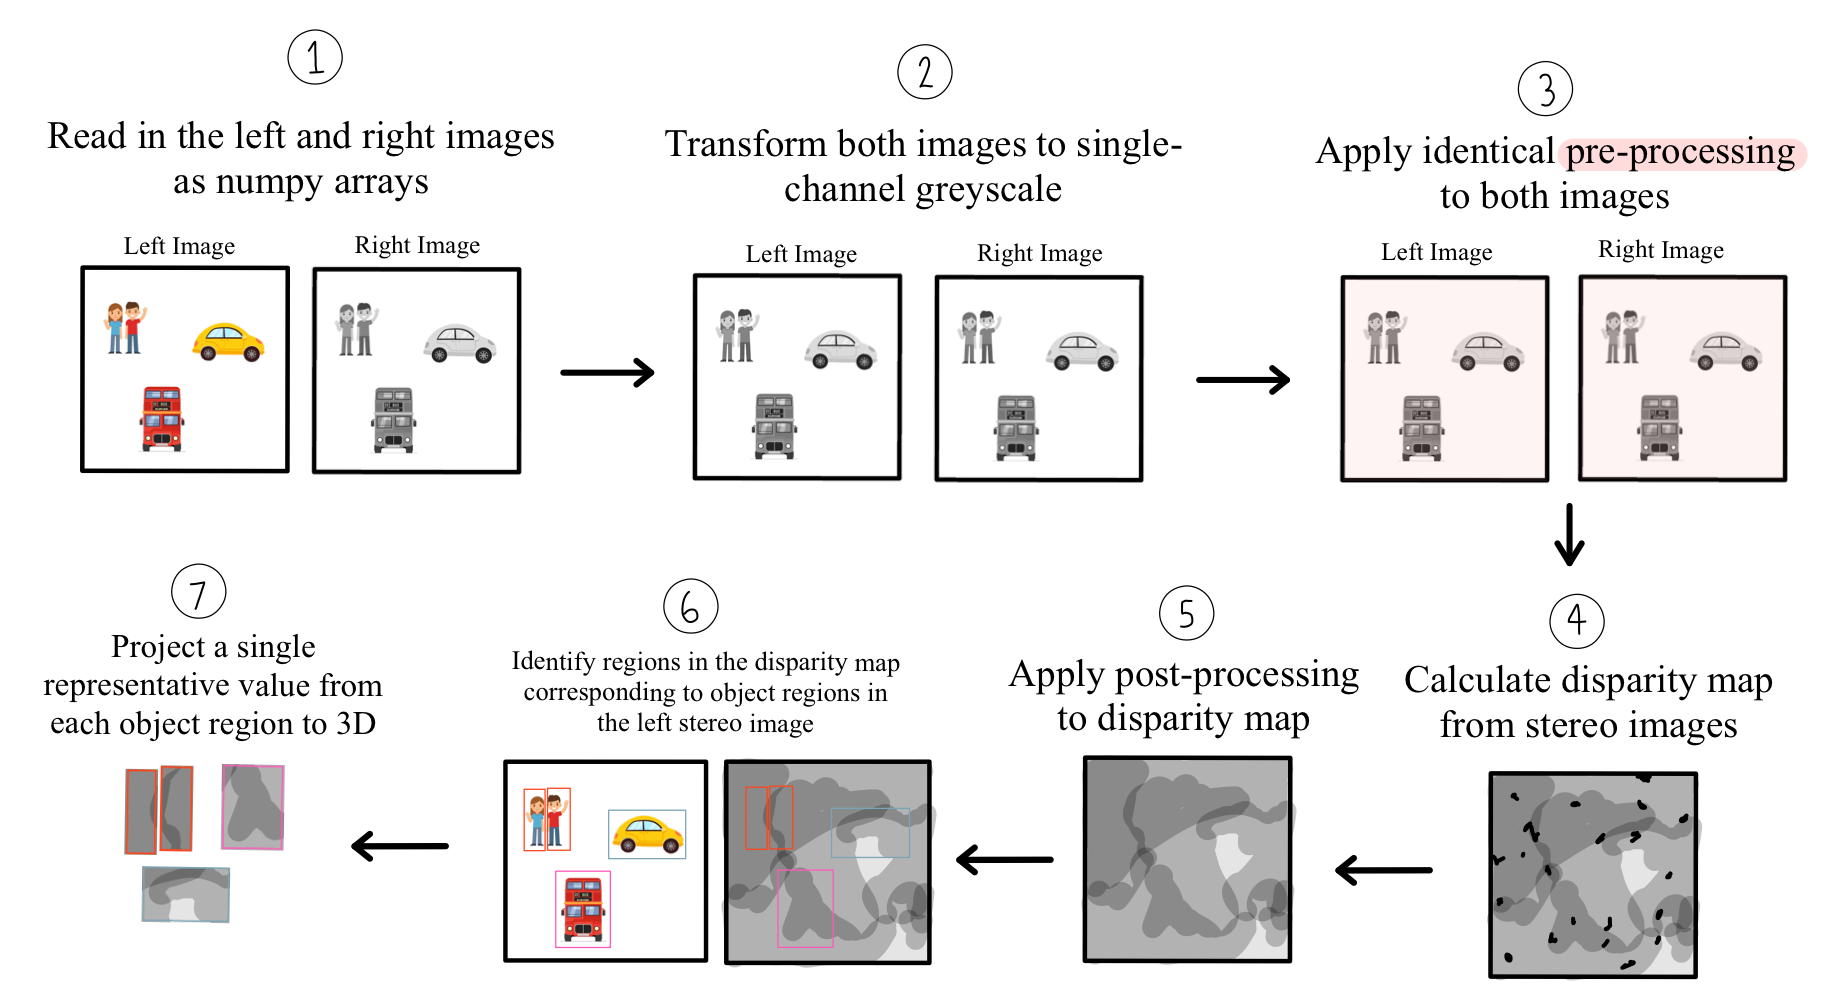
\includegraphics[scale=0.25]{Solutiondiagram}
	\textit{Figure 1: Solution overview}
\end{center}


\newpage



\section{Solution Design}
\noindent There exists an extensive body of literature covering machine learning and deep learning approaches to natural language processing problems, however in the application domain of sarcasm detection, they mostly display low accuracy. This could be due, in part, to the absence of a concrete, all-encompassing definition of sarcasm. N.B. this may also contribute to poor human accuracy in detecting a fundamentally human construct. \\


\bibliography{projectpaper}


\end{document}